\documentclass[12pt]{article}
\usepackage{amsmath}
\usepackage[linesnumbered,ruled]{algorithm2e}
\usepackage[noend]{algpseudocode}
\usepackage{graphicx}
\usepackage{hyperref}
\usepackage{tikz,forest}
\usetikzlibrary{arrows.meta}
\usepackage{forest}
\usepackage{adjustbox}
\usepackage{skmath}
\usepackage{inputenc}
\usepackage{amsmath,amsthm,amssymb}
 \usepackage{tabu}
 \usepackage{graphicx}
\usepackage{wrapfig}
\graphicspath{ {images/} }
\usepackage{tcolorbox}
\newtheorem*{remark}{Remark}

\makeatletter
\def\BState{\State\hskip-\ALG@thistlm}
\makeatother

\forestset{
    .style={
        for tree={
            base=bottom,
            child anchor=north,
            align=center,
            s sep+=1cm,
    straight edge/.style={
        edge path={\noexpand\path[\forestoption{edge},thick,-{Latex}] 
        (!u.parent anchor) -- (.child anchor);}
    },
    if n children={0}
        {tier=word, draw, thick, rectangle}
        {draw, diamond, thick, aspect=2},
    if n=1{%
        edge path={\noexpand\path[\forestoption{edge},thick,-{Latex}] 
        (!u.parent anchor) -| (.child anchor) node[pos=.2, above] {Y};}
        }{
        edge path={\noexpand\path[\forestoption{edge},thick,-{Latex}] 
        (!u.parent anchor) -| (.child anchor) node[pos=.2, above] {N};}
        }
        }
    }
}


\begin{document}

\noindent
{\large{ \textbf{Reinforcement Learning} }}\\

\noindent
\textsl{1. Introduction to reinforcement learning}\\

\noindent
\textsl{1.1 Why reinforcement learning:}\\
There are problems where we can formulate them as MDP, but we are unsure of its transition model $T$ and reward function $R$. If we know its $T$, and $R$, then we can either run policy iteration or value iteration to obtain an optimal policy. However, when T/R, or T and R, are unknown, we can utilize reinforcement learning.  \\

\noindent
\textsl{1. 2 Goal of reinforcement learning:}\\
Agent learns to act optimally, i.e. learn to maximize expected rewards, by receiving feedbacks in the form of rewards. 
\begin{remark}[Utility]
 Agent's utility is defined by the reward function. \\
\end{remark}
\noindent
\textsl{1.3 Types of reinforcement learning:}
\begin{itemize}
\item \textbf{Passive learning}: also referred as `prediction'. We evaluate a fixed policy, instead of learning good actions. 
\item \textbf{Active learning}: learning to act optimally
\end{itemize}
\noindent
Each of the above section, can be further divided into: 
\begin{itemize}
\item \textbf{Model-based learning:} learn the model of MDP, i.e. learn the transition probability model $T(s, a, s')$, and observe $R(s, a, s')$ from experience of $(s, a, s')$. Compute optimal policy by either value iteration or policy iteration.
\item \textbf{Model-free learning:} Bypass the need to learn $T$, $R$, compute an optimal policy from experience of agent its own, or other policies with a Q-learning table, which records state-action values. Passive model-free learning are TD, MC.  Active model-free learning can be classified into:
\begin{itemize}
\item \textbf{On-policy learning:} Learn about policy $\pi$ from experience sampled from $\pi$, e.g. SARSA
\item \textbf{Off-policy learning:} Learn about policy $\pi$ from experience sampled from $\mu$, e.g. Q-learning
\end{itemize}
\end{itemize}

\begin{remark}[Optimal Policy]
Optimal policy is deterministic.
\end{remark}
\begin{remark}[$\pi$, $\mu$]
\end{remark}

\noindent
\textsl{1.4 Definitions}
\begin{itemize}
\item \textbf{Model:} We refer model as transition probability model, $T$.\\

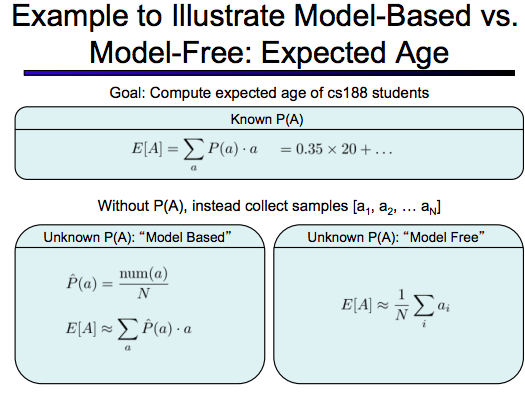
\includegraphics[scale=0.6]{model}\\
\end{itemize}


\noindent
\textsl{2. Passive reinforcement learning}\\

\noindent
In passive learning, the policy is fixed. Therefore, we only learn the utility value of each state if the policy is run from that state. The \textbf{goal} is to learn the value function $U^\pi (s)$ from observations when \textbf{transition model} $P(s' | s, a)$ and \textbf{reward function} $R(s)$ are unknown.  \\

\begin{tcolorbox}
General idea:
\begin{itemize}
\item The agent executes a set of trials using the fixed policy $\pi$.
\item The utility or value for $\pi$ is $U^\pi (s) = E[\sum_{t=0}^{\infty} \gamma ^t R(s_t)]$
\end{itemize}
Question: how to compute $U^\pi (s)$?
\end{tcolorbox}

\noindent
\textsl{2.1 Model-based leaning:}
\begin{itemize}
 \item Adaptive Dynamic Programming: learns the $T$, $R$ model, then solves it. 
 \begin{itemize}
 \item Learn the transition probabilities $P(s' | s, \pi(s))$
 \item Learn reward function $R(s)$
 \item Calculate the value by solving the \textbf{Bellman equation} with linear algebra
 \begin{itemize}
  \item Can use \textbf{modified policy iteration} method of doing k iteration of value updates after each change to model
 \end{itemize}
  \item Can learn the model using supervised learning. The pseudo-code below shows learning using maximum likelihood with table representing $P(s | s, a)$
 \end{itemize}
 

\end{itemize}

\noindent
\textsl{2.2 Model-free leaning:}
\begin{itemize}
 \item Direct Utility Estimation / Monte Carlo Learning 
  \begin{itemize}
  \item \textbf{Expected reward-to-go/return:} In a state, the utility or value is the expected total reward from that state onwards
  \item Each trial is treated as providing a sample of this quantity for each state visited 
  \item Keep \textbf{a running average} for each state in a table. In infinitely many trial, sample average will converge to expected value.
 
  \begin{itemize}
  \item Running average: 
  
\begin{equation} \label{eq1}
\begin{split}
U_k (s) & = \frac{1}{k} \sum_{i=0}^{k} G_i(s)  \\
 & = \frac{1}{k} (G_k (s) + (k-1) G_{k-1} U_{k-1}(s)\\
 & = \underbrace{U_{k-1} (s)}_{\text{Estimate after k-1 returns}}+ \frac{1}{k} \underbrace{(G_k (s) - U_{k-1} (s))}_{\text{Prediction Error}} \\
\end{split}
\end{equation}
\end{itemize}
  \item Monte Carlo Learning is just an instance of supervised learning: each example has state as inout and observed return as output
   \item Advantage: Simple; Each labeled target/return is an unbiased estimate
   \item Disadvantage: 
    \begin{itemize}
    \item Need to wait till the end of episode before learning can be done
    \item Variance can be high as a return is a sum of many rewards over the sequence. Exploiting the constraint imposed by the Bellman equation may help reduce variance ($\implies$ Temporal-Difference Learning)
    \end{itemize}
   
 \end{itemize}
\item \textbf{Temporal difference} learning exploits more of the Bellman equation constraints than Monte Carlo learning. For a transition from state $s$ to $s'$, TD learning does:
 $U^\pi (s) = U^\pi (s) + \alpha( \underbrace{R(s) + \gamma U^\pi(s') - U^\pi(s))}_{\text{TD Error}}$ 
\begin{itemize}
\item $\alpha$ is the learning rate
\item $R(s) + \gamma U^\pi(s')$ is called the TD target
\item $R(s) + \gamma U^\pi(s') - U^\pi(s)$ is called the TD error
\item Converges to the expected value if $\alpha$ decreases with the number of times the states has been visited, e.g. $\alpha (n) = O(1/n)$
\end{itemize}

\end{itemize}


\begin{remark}[Model-free]
TD does not need a transition model to do the updates, only the observed transition.
\end{remark}

\noindent
\textsl{2.3 n-step TD}
\begin{itemize}
\item Let $G_{t:t+n} = R_t + \gamma R_{t+1} + \gamma^2R(r+2) + ... + \gamma ^n \overline{V}(S_{t+n})$, where $\overline{V}(S_{t+n}$ is the estimated value at state $S_{t+n}$
\item n-step TD sets $G_{t:t+n}$ as the target for update
\end{itemize}

\noindent
\textsl{2.4 TD($\lambda$)}
\begin{itemize}
\item $G_t^ \gamma = (1 - \lambda) \sum_{n=1}^{\infty} \gamma ^{n-1} G_{t:t+n}$, an average TD value over different values of n. 
\item $G_t^ \gamma$ is a weighted sum of n-step returns, where n-th step is weighted by $\lambda ^{n-1}$ 
\item When $\lambda=1$, we get Monte Carlo. When $\lambda = 0$, we get TD. \\
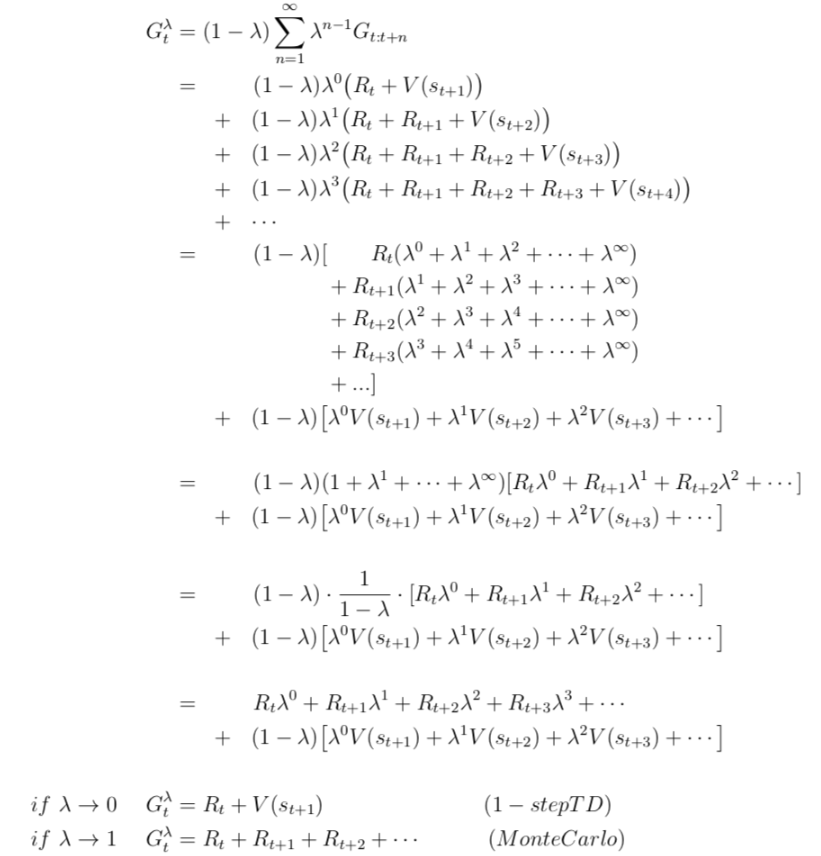
\includegraphics[scale=0.42]{td}\\
\end{itemize}

\noindent
\textsl{2.5 Summary}\\

\textbf{TD vs. ADP}
\begin{itemize}
\item ADP learns the model then solves for $U^\pi(s)$ for each state
\item TD/MC does not need a model. They can work with measurements from the real world, or a simulator. 
\item ADP tend to be more data efficient - requires less data from the real world
\item TD does not need to compute expectation, does not need to solve the system of linear equations - tend to be computationally more efficient.
\end{itemize}



\textbf{TD vs. MC}

\begin{itemize}
\item TD can learns/updates after every step. MC learns/updates after each episode. 
\item TD target depends only on one measured reward. MC target $G(s)$depends on the sum of many rewards.
\begin{itemize}
\item TD target has low variance but is biased
\item MC target is unbiased but has higher variance
\end{itemize}
\item TD usually converges faster than MC in practice because TD exploits constraints of the Bellman equation
\end{itemize}



\textbf{Model-based  vs. Model-free}\\

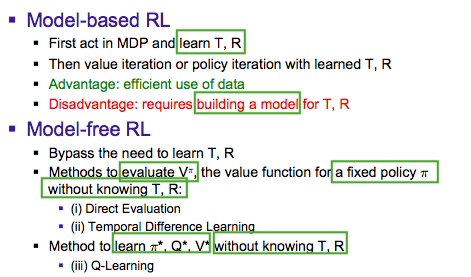
\includegraphics[scale=0.63]{models}\\



\noindent
\textsl{3. Active reinforcement learning}\\

\noindent
Actions in reinforcement learning not only gain rewards but also help learn a better model. By improving the model, greater reward may potentially be obtained. Therefore there is a need between:

\begin{itemize}
\item Exploitation: maxmize value as reflected by the current estimate/current utility function
\item Exploration: learn more about the model/model of the world to potentially improve long term well being
\end{itemize}
\noindent
A scheme for balancing exploration and exploitation must:

\begin{itemize}
\item Try each action in each state an unbounded number of times to avoid a finite probability of missing an optimal action
\item Eventually become greedy in the limit of infinite exploration
\end{itemize}
\noindent
Such schemes are greedy in the limit exploration (\textbf{GILE}), e.g. $\epsilon$-greedy is GILE if $\epsilon$ reduces to 0 at $\epsilon_k$ = $\frac{1}{k}$. 

\begin{remark}[$\epsilon$-greedy exploration]
Choose the greedy action with probability (1 - $\epsilon$), and an action from the policy with probability $\epsilon$.
\end{remark}
\begin{remark}[$\epsilon$]
The decreasing of $\epsilon$ is important to the convergence of an optimal value.
\end{remark}

\noindent
\textsl{3.1 Greedy action selection with $U^+(s)$}\\

\noindent
GLIE based  $\epsilon$-greedy convergence may be slow, an alternative way to balance exploration and exploitation 
 is to use greedy action selection with respect to an \textbf{optimistic} estimate of the utility $U^+(s)$.\\
 
 \begin{tcolorbox}
$U^+(s) = R(s) + \gamma \operatorname*{arg\,max}_a { f(\sum_{s'}^{} P(s' | s, a) U^+(s'), N(s, a))}$ 
 \end{tcolorbox}
 \noindent
 $N(s, a)$ is the number of times action $a$ has been tried in state $s$.\\

\noindent
\textsl{3.2 Learning Q-value and Q-function}\\

\noindent
Instead of learning teh utility function, we can learn an action-utility function $Q(s, a)$, the value of doing action $a$ in state $s$. \\

\begin{tcolorbox}
Q-values are related to utility values by: $U(s) = \operatorname*{arg\,max}_a{Q(s, a)}$\\

The Q-function similarly satisfies a version of the Bellman equations: $Q(s, a) = R(s) + \gamma \sum_{s'}^{} P(s' | s, a)  \operatorname*{arg\,max}_{a'}{Q(s', a')}$
\end{tcolorbox}

\begin{itemize}
\item Model-based: take ADP approach, learn P(s' | s, a), then use an iterative method to compute the Q-function, given the estimated model. 
\begin{itemize}
\item ADP with Q-learning still need model for learning but not to take actions
\item Using MC/TD do not need model for learning and taking actions
\end{itemize}

\item Model-free: an agent that learns a Q-function does not need a model of the form P(s' | s, a) for action selection.
\end{itemize}

\noindent
\textsl{3.3 GLIE $\epsilon$-greedy MC control}\\

\noindent
\textsl{3.3.1 $\epsilon$-greedy exploration}
\begin{itemize}
\item Simplest idea for ensuring continual exploration
\item All $m$ actions are tried with non-zero probability / every action has a non-zero probability to be tried
\item With probability $\epsilon$ choose an action at random:\\
\begin{equation}
    \pi(a|s)=
    \begin{cases}
      \epsilon/m + 1 - \epsilon, & \text{if}\ a^*= \operatorname*{arg\,max}_{a \in A}{Q(s, a)}\\
      \epsilon/m, & \text{otherwise}
    \end{cases}
  \end{equation}
\end{itemize}

\noindent 

 \begin{tcolorbox}
 $\epsilon$-Greedy Policy Improvement: \\
 
Theorem: For any $\epsilon$-greedy policy $\pi$, the $\epsilon$-greedy policy $\pi '$ with respect to $q_{\pi}$ is an improvement.
 \end{tcolorbox}
 
 \noindent
\textsl{3.3.2 GLIE $\epsilon$-greedy MC control}\\

\noindent
General Idea:
\begin{itemize}
\item Sample $k$th episode using $\pi$: \{$S_1, A_1, R_1, ..., S_T$\} ~ $\pi$
\item For each state $S_t$ and action $A_t$ in the episode, 
\begin{itemize}
\item $N(S_t, A_t) = N(S_t, A_t)+1$
\item $Q(S_t, A_t) = Q(S_t, A_t) + \frac{1}{N(S_t, A_t)}(G_t - Q(S_t, A_t))$
\end{itemize}
\item Improve policy based on new action-value function
\begin{itemize}
\item $\epsilon = \frac{1}{k}$
\item $\pi =\epsilon-greedy(Q) $
\end{itemize}
\end{itemize}
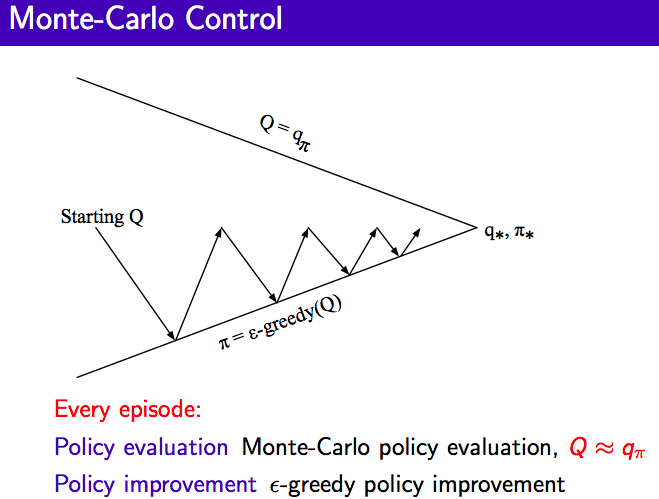
\includegraphics[scale=0.35]{mc2}\\

 \begin{tcolorbox}
Theorem: GLIE Monte-Carlo control converges to the optimal action-value function, $Q(s, a) \Rightarrow q_*(s, a) $
 \end{tcolorbox}
 

\noindent
\textsl{3.4 Q-learning}
\begin{itemize}
\item With TD update, we have what is called Q-learning:\\
$Q(s, a) = Q(s, a) + \alpha(R(s) + \gamma \operatorname*{arg\,max}_{a'}{Q(s', a')} - Q(s, a))$
\item Q-learning is \textbf{off-policy}. Works regardless of policy for generating the trajectory, e.g. random policy
\end{itemize}

\noindent
\textsl{3.4 SARSA}
\begin{itemize}
\item
$Q(s, a) = Q(s, a) + \alpha(R(s) + \gamma {Q(s', a')} - Q(s, a))$ where $a'$ is the action actually taken, whereas in Q-learning, $a$ is the estimated action across different state-action pairs.
\item In comparison, Q-learning uses the max over possible actions $a'$.
\item SARSA is \textbf{on policy}. If agent policy is always exploring, learns to take exploration into account as well.
\item When greedy agent that takes action with best Q-value is used, Q-learning is the same with SARSA.
\item n-step SARSA \\

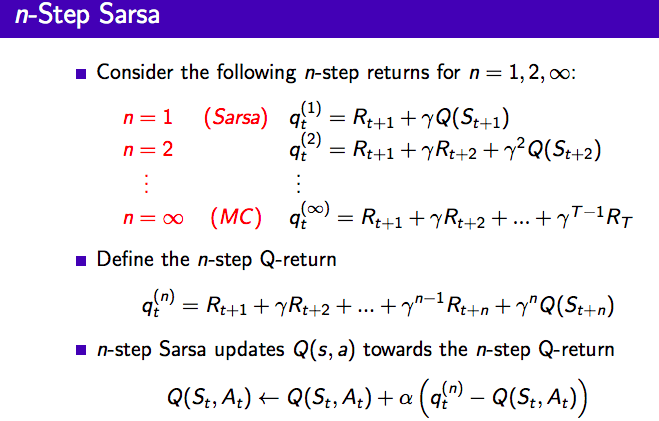
\includegraphics[scale=0.38]{sarsa}\\
\end{itemize}

\noindent
\textsl{3.5 Summary}
\begin{itemize}
\item On-policy: given a policy, while agent follow the given policy, agent evaluate the policy and update the policy on the go.
\item Off-policy: given a behavioural policy, agent evaluates other policies/target policy $\pi(a|s)$ to compute $Q_\pi(s, a)$
\begin{itemize}
\item Learn from observing humans or other agents
\item Re-use experience generated from old policies $\pi_1, \pi_2, ...$
\item Learn about optimal policy while following exploratory policy
\item Learn about multiple policies while following one policy
\end{itemize}
\item MDP \& RL\\

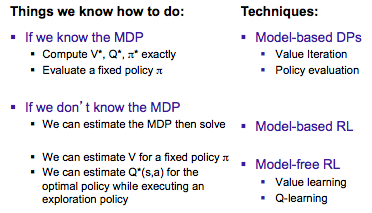
\includegraphics[scale=0.7]{s1}\\

\item DP \& TD\\

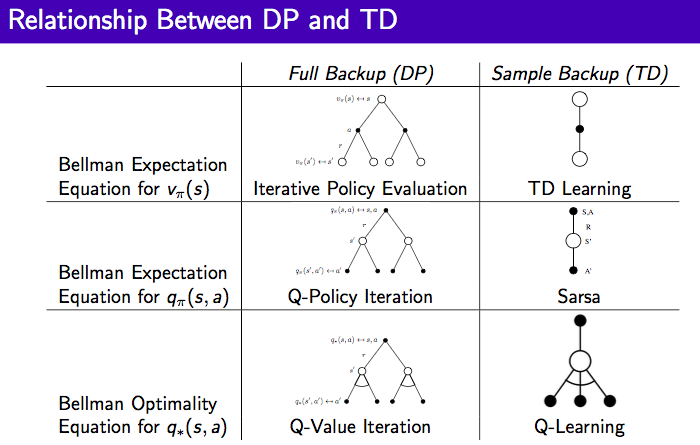
\includegraphics[scale=0.4]{s2}\\
\end{itemize}

\noindent
\textsl{4. Function approximation}\\

\noindent
Function approximation helps to scale reinforcement learning by discarding the Q-table, and generalizing from what the agent has seen to unseen. Here we focus on the \textbf{linear combinations of features} as it is differentiable therefore easier to adjust its parameters by looking at its \textbf{gradient}.  \\

\noindent
For example, $\overline U_{\theta} (s) = \theta_1f_1(s) + \theta_2f_2(s) + ... + \theta_nf_n(s)$, where $\overline U_{\theta} (s)$ is the function approximation that uses $n$ parameters in $\theta$ to weight $n$ features of a state to represent a very large state space. Reinforcement learning agent is supposed to learn $\theta_1, \theta_2 ... $ to approximate the $U(s)$.\\

\noindent
\textsl{4.1. Function approximation with Monte Carlo learning}\\
\begin{itemize}
\item Obtain a set of training samples: $(((x_1, y_1), u_1), ((x_2, y_2), u_2), ..., ((x_n, y_n), u_n ))$, where $u_j$ is the measured utility of the $j$-th example. Note, $u_j$ is unbiased 
\item This gives a \textbf{supervised learning} problem. 
\item With squared error and linear function, we get a standard linear regression problem. 
\item The squared error can be minimized with \textbf{online learning}/stochastic gradient descent.
\item For $j$-th example, the error can be represented as:
\begin{equation} 
\begin{split}
E_j (s) & = (\overline U_\theta(s) - u_j(s))^2  \\
\end{split}
\end{equation}

\item $i$-th parameter $\theta_i$ can be updated as:

\begin{equation}
\begin{split}
\theta_i (s) & = \theta_i \underbrace{-}_{\text{Negative gradient}} \alpha \frac{\partial E_j}{\partial \theta_i}  \\
 & = \theta_i + \alpha (\overline U_\theta(s) - u_j(s)) \frac{\overline U_\theta(s)}{\partial \theta_i} \\
\end{split}
\end{equation}

\end{itemize}

\noindent
\textsl{4.2 Online learning with temporal difference learning :}
\begin{itemize}
\item Obtain a set of training data: $((s_1, (R(s_2)+\gamma U_\theta (s_2))), (s_2, (R(s_3)+\gamma U_\theta (s_3))), ..., (s_n, (R(s_{n+1})+\gamma U_\theta (s_{n+1}))) )$
\item For TD:  $\theta_i = \theta_i + \alpha (R(s) +  \gamma \overline U_\theta(s') - \overline U_\theta(s)) \frac{\partial \overline U_\theta(s)}{\partial \theta_i}$

\item For Q-learning: $\theta_i = \theta_i + \alpha (R(s) +  \gamma  \operatorname*{arg\,max}_{a'} \overline Q_\theta(s', a') - \overline Q_\theta(s, a)) \frac{\partial \overline Q_\theta(s,a)}{\partial \theta_i}$
\end{itemize}

\noindent
\textsl{5. Policy search}\\

\noindent
\textsl{5.1. Policy representation and search}\\

\noindent
\textbf{Policy search} adjusts $\theta$ to improve the policy. Policy search tries to find a policy, e.g. represented as Q-functions that does well, so $Q^*/10$ can given the same optimal actions as $Q^*$. In contrast, Q-learning with function approximation tries to find a value of $\theta$ such that $\overline Q_\theta$ that is close to $Q^*$.\\

\begin{itemize}
\item Use \textbf{stochastic policy} $\pi_\theta(s, a)$ that specifies the probability of selecting action $a$ in state $s$. This solves the problem that policy as a function of action is discontinuous. For example, the \textbf{softmax function}: 

$\underbrace{\pi_\theta (s, a)}_{\text{Probability distribution of actions in s}} = \frac{e^{\overline Q_\theta (s,a)}} { \underbrace{\sum_{a'}^{} e^{\overline Q_\theta (s,a')}}_{\text{Nomalization}} }$
 
 \item We can specify the \textbf{policy value} as $\rho (\theta)$. $\rho (\theta)$ can be optimized by:
 \begin{itemize}
 \item Taking a step in the direction of the \textbf{policy gradient} $\nabla_\theta \rho (\theta)$/hill climbing (positive gradient descent), if $\rho (\theta)$ is differentiable (if we specify the policy in softmax function).
 
 \item Look for a local optimal
 \end{itemize}
 
 \item For stochastic environment and/or policy $\pi_\theta (s,a)$, it is possible to obtain an unbiased estimate of gradient at $\theta$, $\nabla_\theta \rho (\theta)$ directly from results of trials executed at $\theta$.
 
 \item Consider \textbf{single action from single state $s_0$}:
 
  $\nabla_\theta \rho (\theta) = \nabla_\theta  \sum_{a}^{} \pi_\theta(s_0, a) R(a) = \sum_{a}^{} \nabla_\theta(\pi_\theta(s_0, a))R(a)$ \\
  
  Then we approximate the summation using \textbf{samples} generated from $\pi_\theta (s_0, a)$/ sample $N$ samples ($a_n$) from one state:  
 
 $\nabla_\theta \rho (\theta) = \sum_{a}^{} \pi_\theta(s_0, a) \frac{\nabla_\theta(\pi_\theta(s_0, a))R(a)}{\pi_\theta(s_0, a)} \approx \frac{1}{N} \sum_{j=1}^{n} \frac{\nabla_\theta(\pi_\theta(s_0, a_j))R(a_j)}{\pi_\theta(s_0, a_j)}$
 
\end{itemize}

\noindent
\textsl{5.2. Policy search: REINFORCE algorithm}\\

 \begin{itemize}
 \item From \textbf{single state}, we generalize this idea to \textbf{sequential case}: state $s_i$ and action $a_{ij}$, $\pi_\theta(s_i, a_{ij}) $. 
 
 $\nabla_\theta \rho (\theta)  \propto \sum_{s}^{} \rho_{\pi_\theta}(s) \sum_{a}^{} \frac{ \pi_\theta(s_0, a) \nabla_\theta \pi_\theta(s_0, a)Q_{\pi_\theta}(s, a)}{\pi_\theta(s_0, a)}  \approx \frac{1}{N} \sum_{i}^{N} \sum_{j}^{i} \frac{\nabla_\theta \pi_\theta(s_i, a_{ij})G_{ij}(s_i)}{\pi_\theta(s_i, a_{ij})}$, \\
 
 for each state $s_i$ is visited, $a_{ij}$ is executed on $j$-th trial, and $G_{ij}$ is the total reward/return received from state $s_i$ onwards on $j$-th trial.
 
 \item Use online learning/update, we get \textbf{REINFORCE} algorithm: 
 
 $\theta_{j+1} = \theta_{j} + \alpha G_j \frac{\nabla \theta\pi_\theta (s, a_j)}{\pi_\theta (s, a_j)}$\\
 
 As $\nabla_\theta \ln{\pi_\theta (s, a_j)}  = \frac{\nabla \theta\pi_\theta (s, a_j)}{\pi_\theta (s, a_j)}$, we have rewrite our update function as follows: 
 
 $\theta_{j+1} = \theta_{j} + \alpha G_j \nabla_\theta \ln{\pi_\theta (s, a_j)}$, because usually the gradient of natural logarithm of  the policy function is easier to look for than directly from the policy function itself.\\

 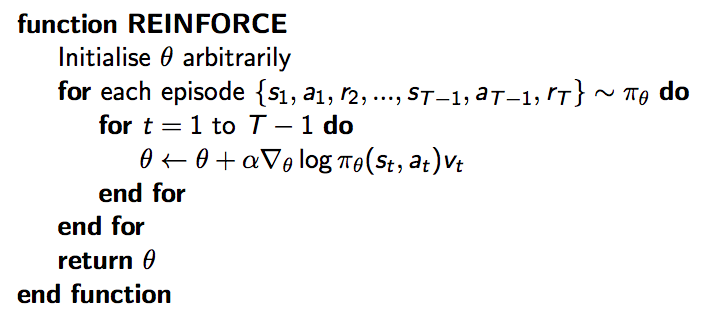
\includegraphics[scale=0.42]{reinforce}\\
 
 
 \item Reduce variance with a \textbf{Baseline}\\
 
  We are estimating $\nabla \rho (\theta) = \sum_{s}{} p_{\pi_\theta} (s) \sum_{a}^{} \nabla_\theta \pi_\theta(s,a_j) Q_{\pi_\theta}(s, a)$
 
 \begin{equation}
\begin{split}
\nabla \rho (\theta) & = \sum_{s}{} p_{\pi_\theta} (s) \sum_{a}^{} \nabla_\theta \pi_\theta(s,a_j) Q_{\pi_\theta}(s, a) \\
 & =  \sum_{s}{} p_{\pi_\theta} (s) \sum_{a}^{} \nabla_\theta \pi_\theta(s,a_j) (Q_{\pi_\theta}(s, a) - B(s))\\
 & =  \sum_{s}{} p_{\pi_\theta} (s) (\sum_{a}^{} \nabla_\theta \pi_\theta(s,a_j) Q_{\pi_\theta}(s, a) - (\sum_{a}^{} \nabla_\theta \pi_\theta(s,a_j)B(s)))\\
  & =  \sum_{s}{} p_{\pi_\theta} (s) (\sum_{a}^{} \nabla_\theta \pi_\theta(s,a_j) Q_{\pi_\theta}(s, a) - B(s)(\underbrace{\sum_{a}^{} \nabla_\theta \pi_\theta(s,a_j)}_{\text{ Distribution sums up to 1}}))\\
  & = \sum_{s}{} p_{\pi_\theta} (s) (\sum_{a}^{} \nabla_\theta \pi_\theta(s,a_j) Q_{\pi_\theta}(s, a) - B(s)(\nabla_\theta 1))
\end{split}
\end{equation}
 
  \begin{itemize}
  \item Using a baseline function B(s) can reduce variance 
  \item Use an \textbf{advantage function} in place of $Q_{\pi_\theta} (s, a)$: $A_{\pi_\theta} (s, a) = Q_{\pi_\theta} (s, a) - V_{\pi_\theta} (s)$, where  $V_{\pi_\theta} (s)$ is the baseline function
  \end{itemize}
 \item REINFORCE uses a Monte Carlo estimate of the advantage function, which has higher variance. To reduce variance, an alternative is to use TD method. The advantage function is: 
  	$Q_{\pi_\theta} (s, a) - V_{\pi_\theta} (s) = E[r + \gamma V_{\pi_\theta}(s')] - V_{\pi_\theta}(s)$. It is also common to use multiple steps of rewards instead of one step in TD. 
\item \textbf{actor-crtitic method} : 
   \begin{itemize}
    \item \textbf{Critic}: Learns a value or Q-function, that is to update parameter $w$, that is used only for evaluation
  \item \textbf{Actor}: Learns a policy (actor) that takes action, that is to update parameters $\theta$ in direction suggested by critic
   \item The critic is solving a familiar problem: policy evaluation
  \item We use a critic to estimate the action-value function, $Q_w (s, a) \approx Q^{\pi_\theta} (s, a)$
  \end{itemize}
 
 \end{itemize}




\begin{algorithm}
    \SetKwInOut{Input}{Input}
    \SetKwInOut{Output}{Output}

    \underline{function PASSIVE-ADP-AGENT(percept) returns an action} \;
    \Input{percept, a percept indicating the current state $s'$ and reward signal $r'$}
    \Output{$a$}
    \textbf{Persistent:} 
    {$\pi$}, a fixed policy; 
    mdp, an MDP with model P, reward R, discount $\gamma$; 
    U, a table of utilities, initially empty; 
    $N_{sa}$, a table of frequencies for state-action pairs, initially zero; 
    $N_{s'|sa}$, a table of outcome frequencies given state-action pairs, initially zero; 
    s, a, the previous state and action, initially null \;
    \If{$s'$ is new}
      {
        $U[s'] = r'$ \;
        $R[s'] = r'$\;
      }
      
      \If{$s$ is not null}
      {
        increment $N_{sa}[s, a]$ and $N_{s'|sa}[s', s, a]$ \;        	
	\ForEach{ t such that $N_{t|sa}[t, s, a]$ is nonzero}{%
     		$P(t  | s, a) = N_{s'|sa}[s', s, a]$ /\ $N_{sa}[s, a]$\;
         }   
      }
      U = POLICY-EVALUATION ($\pi$, U, mdp)\;
       \eIf{$s'$ is Terminal}
      {
        s, a = null \;
        $R[s'] = r'$\;
      }
      {
      s, a = $s'$, $\pi[s']$
      }
      return a
    \caption{Adaptive Dynamic Programming}
\end{algorithm}

\begin{algorithm}
    \SetKwInOut{Input}{Input}
    \SetKwInOut{Output}{Output}

    \underline{function PASSIVE-TD-AGENT(percept) returns an action} \;
    \Input{percept, a percept indicating the current state $s'$ and reward signal $r'$}
    \Output{$a$}
    \textbf{Persistent:} 
    {$\pi$}, a fixed policy; 
    mdp, an MDP with model P, reward R, discount $\gamma$; 
    U, a table of utilities, initially empty; 
    $N_{sa}$, a table of frequencies for state-action pairs, initially zero; 
    s, a, r, the previous state, action, and reward, initially null \;
    
    \If{$s'$ is new}
      {
        $U[s'] = r'$ \;
      }
      
      \If{$s$ is not null}
      {
        increment $N_{sa}[s, a]$ \;        	
	$U^\pi[s] = U^\pi[s] + \alpha( N_{sa}[s])(R(s) + U\pi[s'] - U\pi[s])$
      }
    
       \eIf{$s'$ is Terminal}
      {
        $s, a, r$= null \;
      }
      {
      s, a, r = $s'$, $\pi[s']$, $r$
      }
      return a
    \caption{Temporal-Difference Learning}
\end{algorithm}

\begin{algorithm}
    \SetKwInOut{Input}{Input}
    \SetKwInOut{Output}{Output}

    \underline{function Q-LEARNING-AGENT(percept) returns an action} \;
    \Input{percept, a percept indicating the current state $s'$ and reward signal $r'$}
    \Output{$a$}
    \textbf{Persistent:} 
    {$Q$}, a table of action values indexed by state and action, initially zero; 
    $N_{sa}$, a table of frequencies for state-action pairs, initially zero; 
    s, a, r, the previous state, action, and reward, initially null \;
    \If{$s'$ is Terminal}
      {
        $Q[s', None] = r'$
      }
      
      \If{$s$ is not null}
      {
        increment $N_{sa}[s, a]$ \;        	
	$Q(s, a) = Q(s, a) + \alpha(N_{sa}[s, a])(R(s) + \gamma \operatorname*{arg\,max}_{a'}{Q(s', a')} - Q(s, a))$
      }
      s, a, r = s', $\operatorname*{arg\,max}_{a'}f(Q(s', a'), N(s', a'))$, r' \;
      return a
      \caption{Q Learning}
\end{algorithm}









\end{document}